
\PassOptionsToPackage{unicode}{hyperref}
\PassOptionsToPackage{naturalnames}{hyperref}
\documentclass{beamer} 
%\usepackage{babel}
%\usepackage[utf8]{inputenc}


%%% FONT SELECTION %%%%%%%%%%%%%%%%%
%%% we choose a sans font %%%%%%%%%%
\usepackage{kmath,kerkis} 
%\usepackage[default]{gfsneohellenic} 
%%%%%%%%%%%%%%%%%%%%%%%%%%%%%%%%%%%%

\usepackage{color}
\usepackage{amsmath}
\usepackage{amssymb}

\usepackage{epstopdf}
\usepackage{graphicx}
\graphicspath{{./images/presentation}}

%%
% load TEI-Pel - specific layout
\usepackage{TeiPel_En_Beamer_Layout}
\setTeipelLayout{draft,newlogo}% options: "draft", "newlogo"



% Thesis Info - first page 
	% title
		\title[Gravimetric Sensing Aided by Radiation Cooling]{Gravimetric Sensing Aided by Radiation Cooling}		
    %\author
		\author[Yishai Arieli]{Yishai Arieli}
	% supervisor	
		\supervisor{Supervisor}{Professor John Howell}
	% date
		\presentationDate{May, 2021}


\begin{document}

% typeset front slides
	\typesetFrontSlides

% Your Slides Start here:
\section{Introduction}



% frame 1
\begin{frame}{\hypertarget{frame:Gravitational field}{Gravitational field}}
	\begin{center}		
		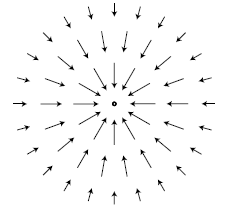
\includegraphics[width=0.3\textwidth,keepaspectratio]{gravity.png}
    \end{center}
	\begin{itemize}
		\item The field vectors point towards the mass: $\overrightarrow{g}(M) = \frac{GM}{r^2}\hat{r}$ .
		\item Since the gravitational constant is small, the force is weak.
		\item Mass vibrations results with energy spectral density.
		\item High sensitivity is a significant challenge at low frequencies.
		\end{itemize}
\end{frame}

% frame 2
\begin{frame}{Previous achievements}
	\begin{center}		
		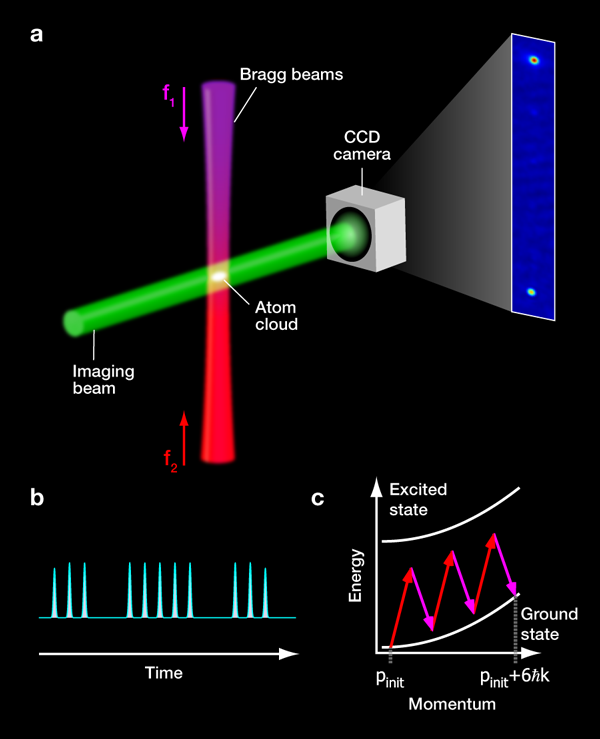
\includegraphics[width=0.3\textwidth,keepaspectratio]{kasevich.png}
	\end{center}
	\begin{itemize}

		\item Interference fringe changes due to free fall in one arm; sensitivity of 100 $\frac{nano-g}{\sqrt{Hz}}$.
		%\item Atomic interferometry; sensitivity of of 100 pico-g after two days of integration.
		\item Superconducting sphere suspended in a magnetic field; sensitivity of 1 $\frac{nano-g}{\sqrt{Hz}}$ after a year of integration
		\item Atom interferometer; sensitivity of 500 femto-g after one hour of integration.

		
	\end{itemize}
\end{frame}

% frame 4
\begin{frame}{\hypertarget{frame:Cavendish apparatus}{Cavendish apparatus}}
	\begin{center}		
		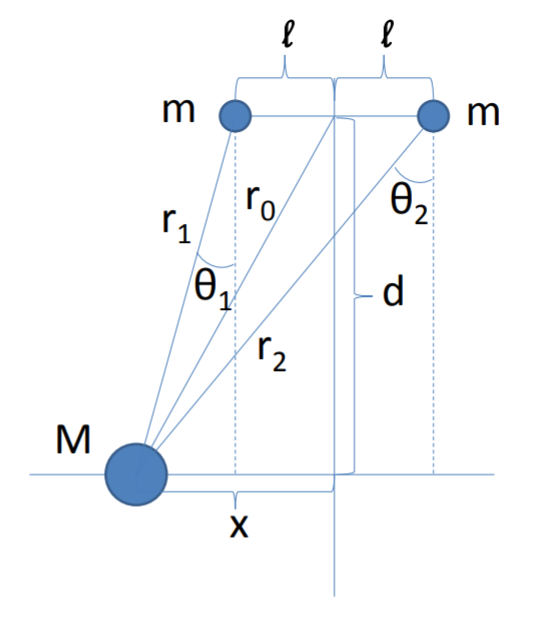
\includegraphics[width=0.25\textwidth,keepaspectratio]{Cavendish apparatus.PNG}
    \end{center}
	\begin{itemize}
		\item Torsional pendulum is an angular harmonic oscillator with a restoring torque, made of a mass hung by a string. 
		\item Apparatus measures the gravitational torque of test mass.
		\item Mass attracts both masses $m$; creating a net torque $\tau_g$.
		\item The average equilibrium angle: $\overline{\theta}_g = \frac{\tau_g}{\kappa} \approx \frac{3GT^2cos\theta sin\theta}{4\pi^2 } \cdot \frac{M}{r_0^3}$.

	\end{itemize}
	\hyperlink{frame:Cavendish apparatus 1}{>>} 
\end{frame}

% frame 3
\begin{frame}{\hypertarget{frame:Harmonic oscillator}{Harmonic oscillator}}
	\begin{center}		
		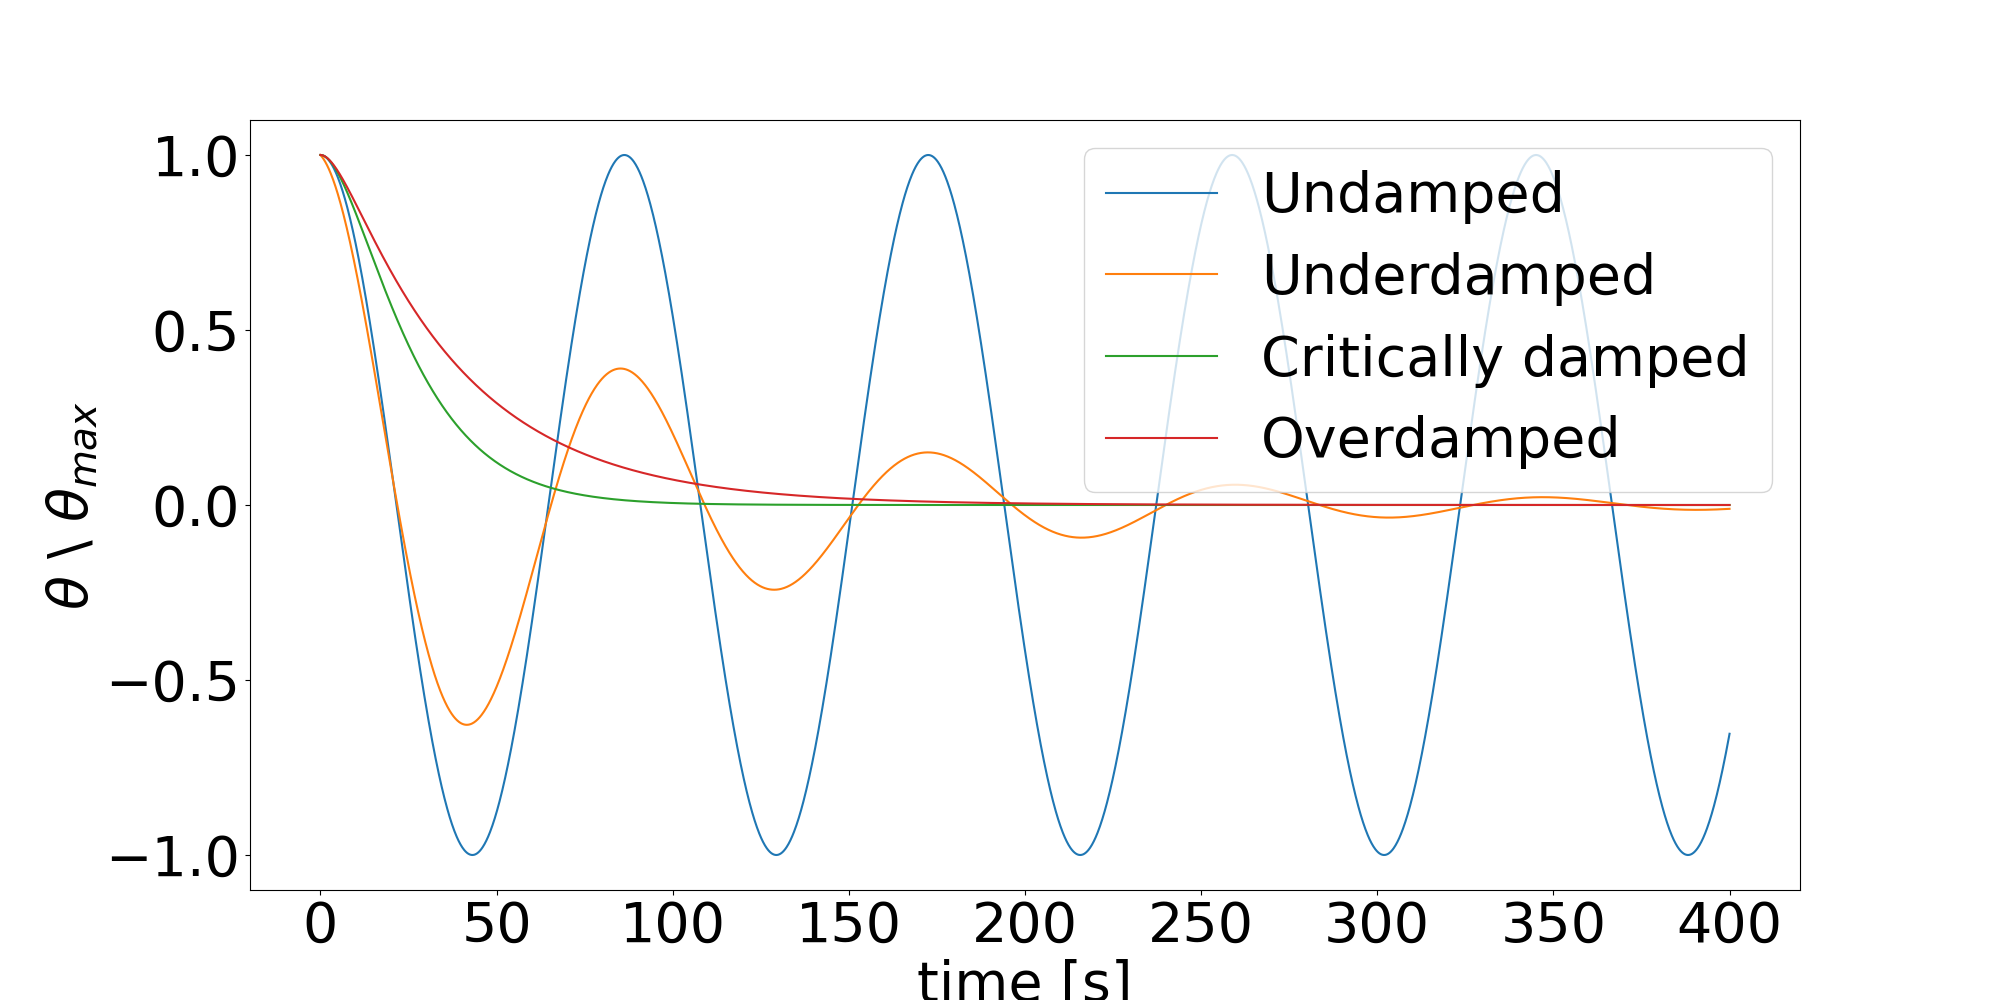
\includegraphics[width=0.55\textwidth,keepaspectratio]{damp.png}
    \end{center}
	\begin{itemize}

		\item Undamped oscillator; harmonic oscillations without decay.
		\item Damped oscillator; there is a damping torque $\tau = \gamma\dot{\theta}(t)$.
		\item Driven oscillator; there is also a time-dependent torque $\tau(t)$.
		
	\end{itemize}
	\hyperlink{frame:Damped oscillator}{>>}
\end{frame}


% frame 1
\begin{frame}{\hypertarget{frame:Measurement uncertainty}{Measurement uncertainty}}
	\begin{center}		
		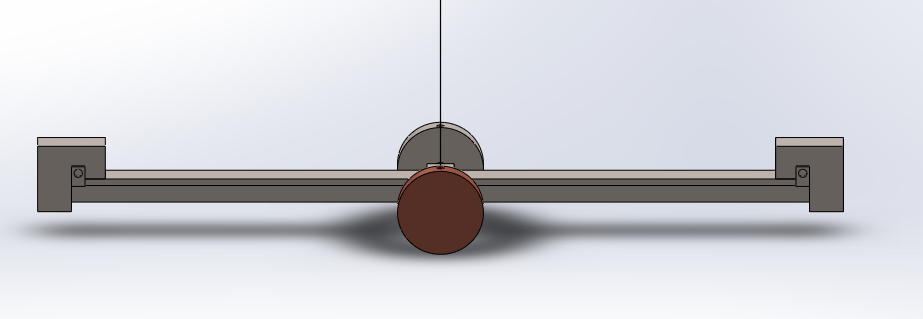
\includegraphics[width=0.4\textwidth,keepaspectratio]{pendulum_front.png}
    \end{center}
	\begin{itemize}
		
		\item Angle is measured using a mirror and quadrant detector.
		\item Fundamental limits are: thermal uncertainty, shot noise. 
		\item Damping effectively lowers the temperature; $\delta\theta = \sqrt{\frac{k_B T}{\kappa}}$. 
		\item Reducing the uncertainty by damping enables higher sensitivity; $\frac{M}{r_0^3} \propto [\overline{\theta}_g\pm \delta\theta] \propto [\overline{\theta}_g\pm \theta_{damped}]$.

		
	\end{itemize}
	\hyperlink{frame:Measurement uncertainty 1}{>>} 
\end{frame}
\section{Methods and results}
\subsection{System structure}
% frame 1
\begin{frame}{\hypertarget{frame:Radiation tourqe}{Radiation tourqe}}
	\begin{center}		
		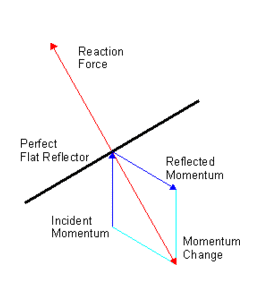
\includegraphics[width=0.2\textwidth,keepaspectratio]{radiation.PNG}
    \end{center}

	
	\begin{itemize}		
		
		\item Incident light beam causes force on the surface, due to momentum exchange with the electromagnetic field.
		\item Two light sources hitting the sides of the pendulum result with power-depended net tourqe.
		\item Power modulation is controlled by a feedback loop.
		
	\end{itemize}
	\hyperlink{frame:Radiation tourqe 1}{>>} 
\end{frame}
\begin{frame}{Experiment setup}
	\begin{center}		
			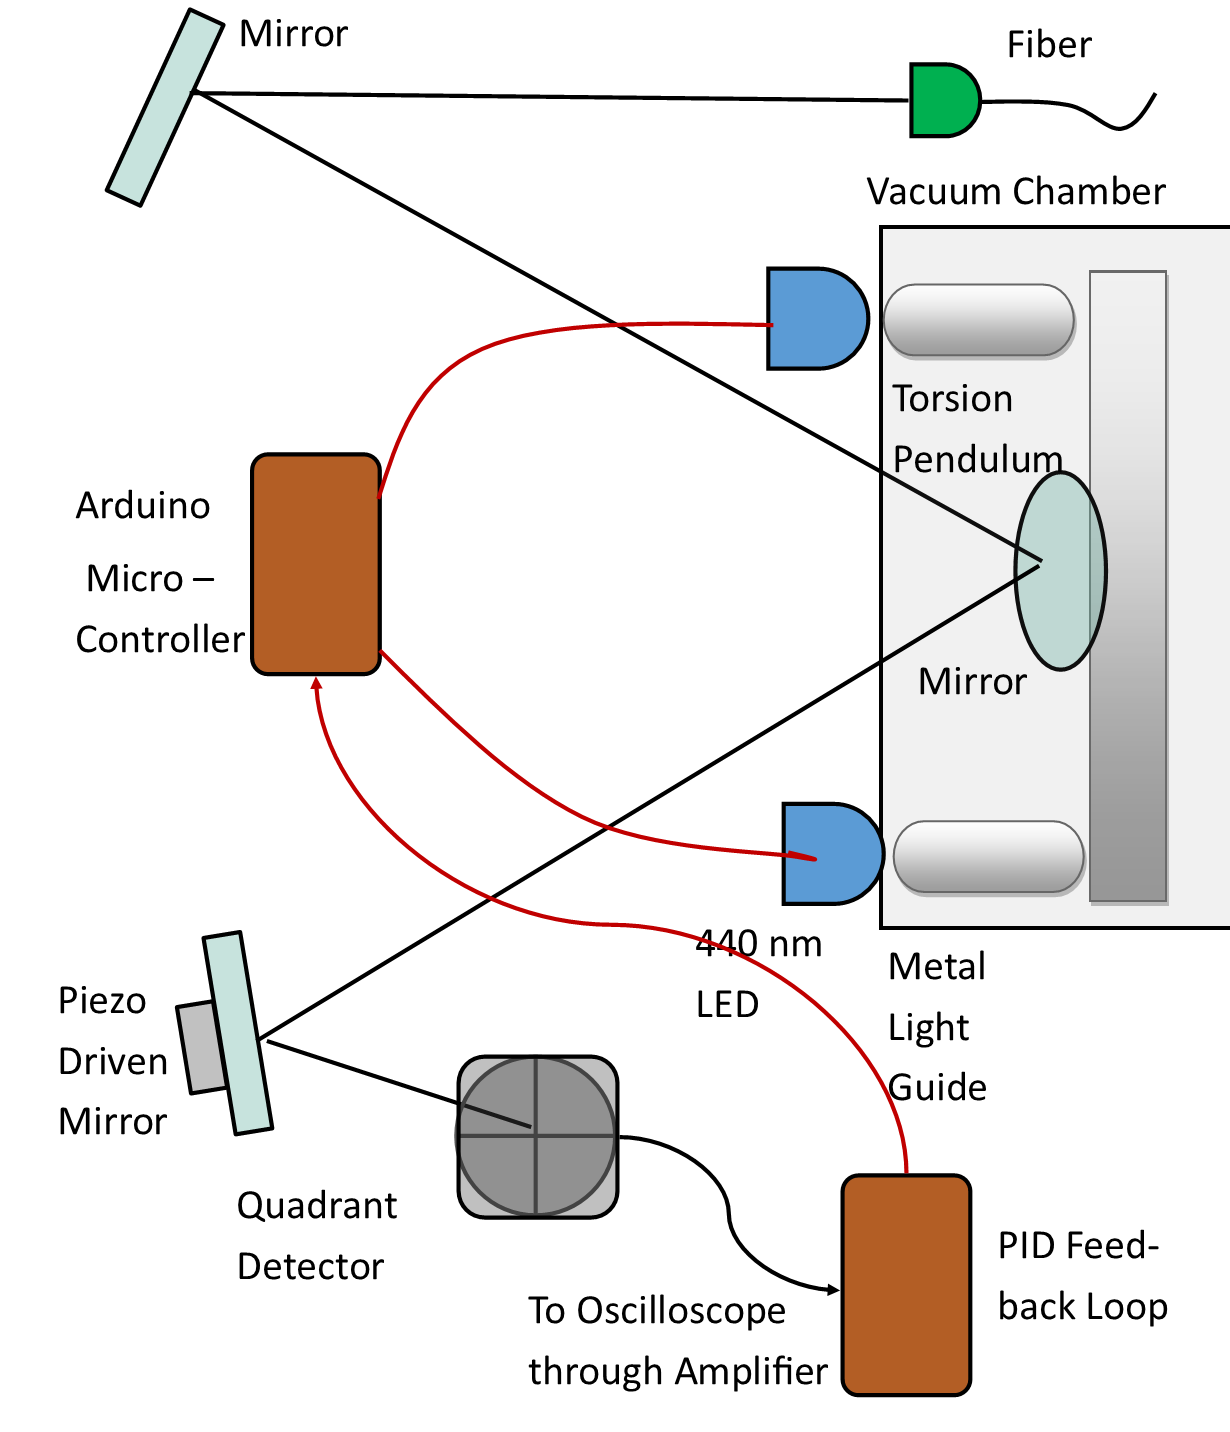
\includegraphics[width=0.3\textwidth,keepaspectratio]{setup cropped.png}
	\end{center}
	\begin{itemize}
		\item Torsional pendulum is placed inside a vacuum chamber and an acoustic box; reducing environmental coupled noises.
		\item A PID algorithm modulates two light sources in real-time.
		\item Pendulum damped by external radiation pressure tourqe.
	
	\end{itemize}
	
\end{frame}

% frame 3
\begin{frame}{Vacuum chamber}
	\begin{center}		
		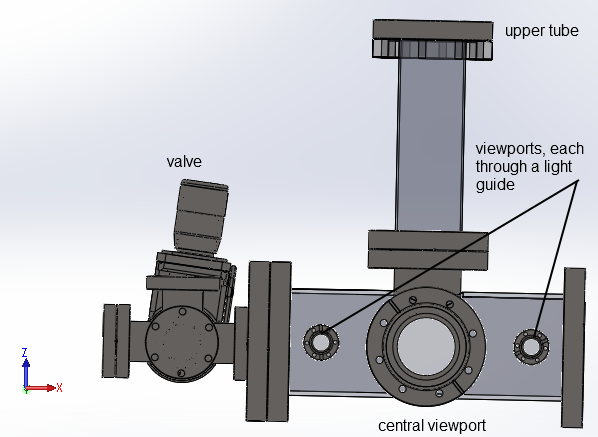
\includegraphics[width=0.4\textwidth,keepaspectratio]{chamber_front_names.PNG}
	\end{center}
	\begin{itemize}
		\item Chamber is with transparent windows through light guides.
		\item Measurements is conducted with vacuum engine off.
		\item Maintenance of low pressure; leakage, outgassing.
		\item Chosen materials minimize magnetic noise and outgassing.

		
	\end{itemize}	
\end{frame}


% frame 4
\begin{frame}{Torsional pendulum}
	\begin{center}		
		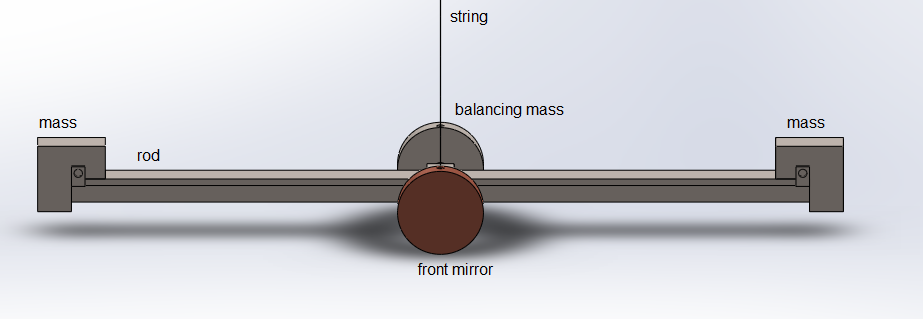
\includegraphics[width=0.4\textwidth,keepaspectratio]{pendulum_front_names.png}
	\end{center}
	\begin{itemize}
		\item Held by an adjustable mount; for accurate location. 
		\item Front mirror stabilized by a balancing mass.
		\item Chosen dimensions aim achieving small $\kappa$ with large $T$.
		\item Measured: $T = 84[s]$, $\kappa = 2.7\cdot10^{-6}[\frac{N\cdot m}{rad}]$.
	\end{itemize}
	\hyperlink{frame:Cavendish apparatus}{<<} 

	
\end{frame}




\subsection{Damping and measurement}

% frame 2
\begin{frame}{\hypertarget{frame:Proportional–integral–derivative (PID) controller}{Proportional–integral–derivative (PID) controller}}
	\begin{center}		
		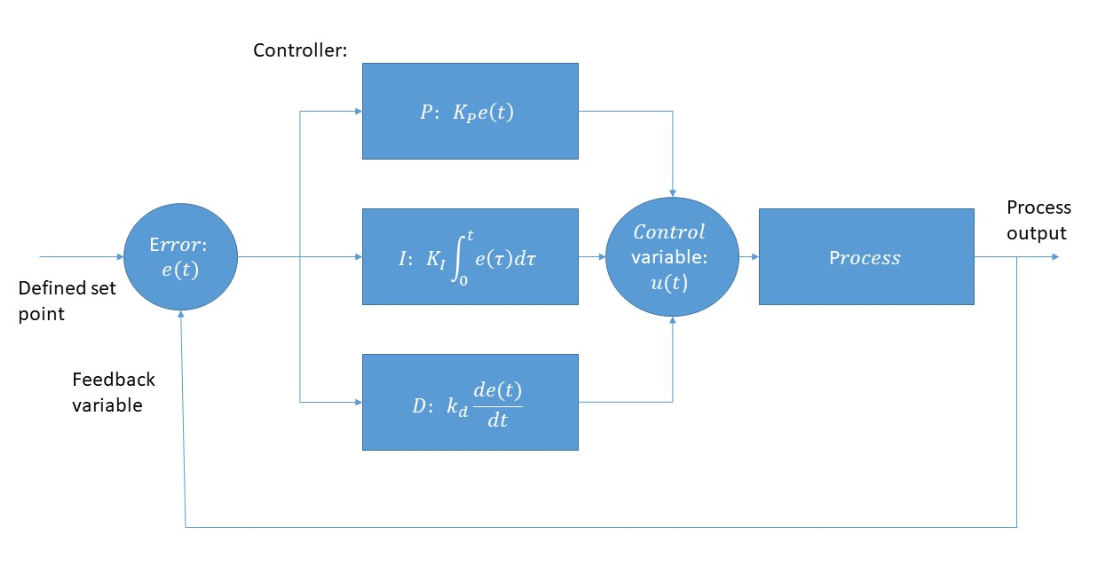
\includegraphics[width=0.6\textwidth,keepaspectratio]{pid_diagram_powerpoint.jpg}
    \end{center}
	\begin{itemize}	
		\item PID controller is a feedback based control system, for time continuous control of a process (damped motion).
		\item The control is a weighted sum of proportional, integral and derivative response to error from defined set point (P-I-D).
		\item Feedback applies an external correction to the process: $\tau(t)$.
		\item When PID tuned correct; critical damping of process.

	\end{itemize}
	\hyperlink{frame:Proportional–integral–derivative (PID) controller 1}{>>} 
\end{frame}

% frame 3

\begin{frame}{Damped motion}
	\begin{center}		
		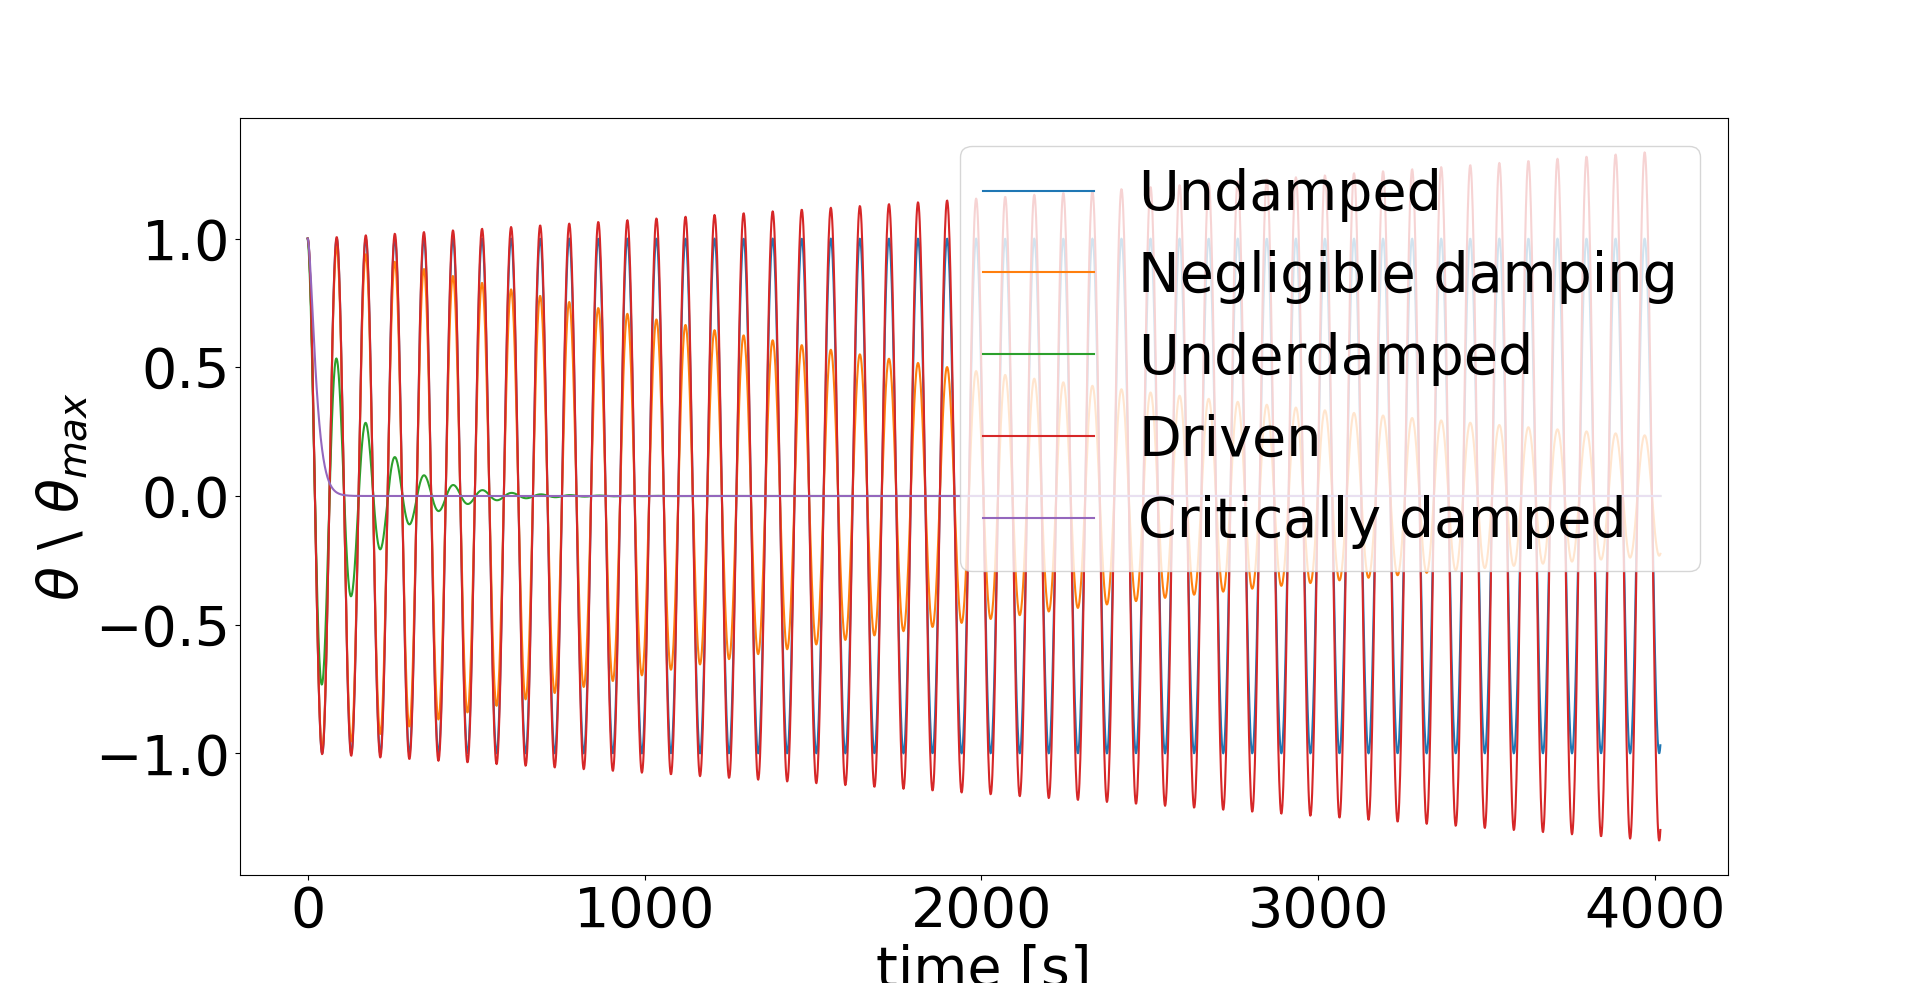
\includegraphics[width=0.65\textwidth,keepaspectratio]{underdamp.png}
	\end{center}
	\begin{itemize}		
		\item PID mainly acts as friction, gradually slowing velocity.
		\item $\tau(t) =  \gamma\dot{\theta}(t) =  \gamma\frac{2\pi}{T} \theta( t) \rightarrow \gamma  =\frac{\tau}{\theta}\cdot \frac{ T}{2\pi} $
		\item Overshoot or slow response; result with driven oscillator.
		\item Torque small compared to amplitude; negligible damping. 
		
	\end{itemize}
\end{frame}

\begin{frame}{\hypertarget{frame:Gravimetric measurement}{Gravitational measurement}}
	\begin{center}		
		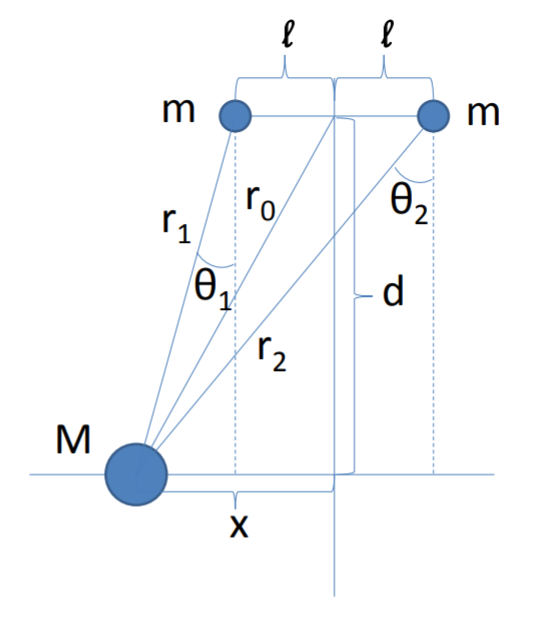
\includegraphics[width=0.3\textwidth,keepaspectratio]{Cavendish apparatus.PNG}
    \end{center}
	\begin{itemize}
		
		\item Introducing a new mass changes equilibrium into $\theta_g(t)$. 
		\item Since motion is damped; PID response is an inverse torque. 
		\item When integrating over short periods: $\overline{\theta}_g =  \frac{\int \tau(t) dt}{ K_P \Delta t} $. 	
		\item Result with lower uncertainty and short integration time.
	\end{itemize}
\end{frame}





\begin{frame}{Previous laser setup}
	\begin{center}		
		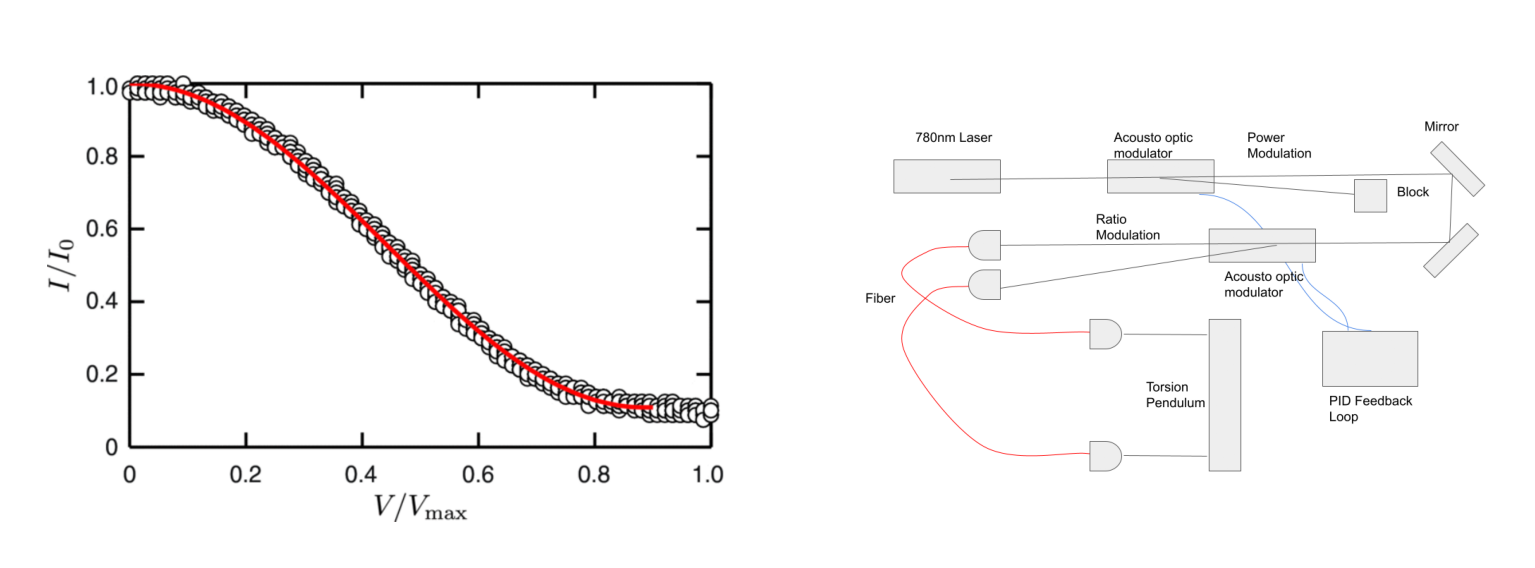
\includegraphics[width=0.8\textwidth,keepaspectratio]{aom2.png}
	\end{center}
	\begin{itemize}		
		\item Laser coupled in series into two acousto optic modulators; divided into two controlled beams with mutual source.
		\item High modulation range of 13-bit.
		\item Non linear response results with uncertainty and overshoot.
		\item Slow frequency causes phase delay; $f \approx 1 [Hz]$.
		%\item Fluctuations uncertainty minimized; mutual source.
	\end{itemize}
\end{frame}

\begin{frame}{\hypertarget{frame:LED PWM setup}{LED PWM setup}}

	\begin{center}		
		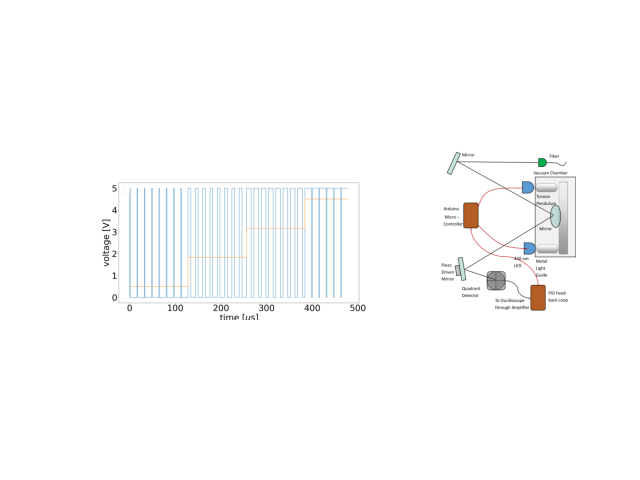
\includegraphics[width=0.55\textwidth,keepaspectratio]{led_setup.png}
	\end{center}
	\begin{itemize}		
		\item LED driven by a PWM circuit using an Arduino controller and coupled into a light guide reducing field of view.
		\item Low modulation range of 8-bit.
		\item Linear response minimizes overshoot.
		\item Fast frequency minimizes phase delay; $f \approx 500[Hz]$.
		
		
	\end{itemize}
	\hyperlink{frame:LED PWM setup 1}{>>} 
\end{frame}


\subsection{Results}
\begin{frame}{Damping result}
	\begin{center}		
		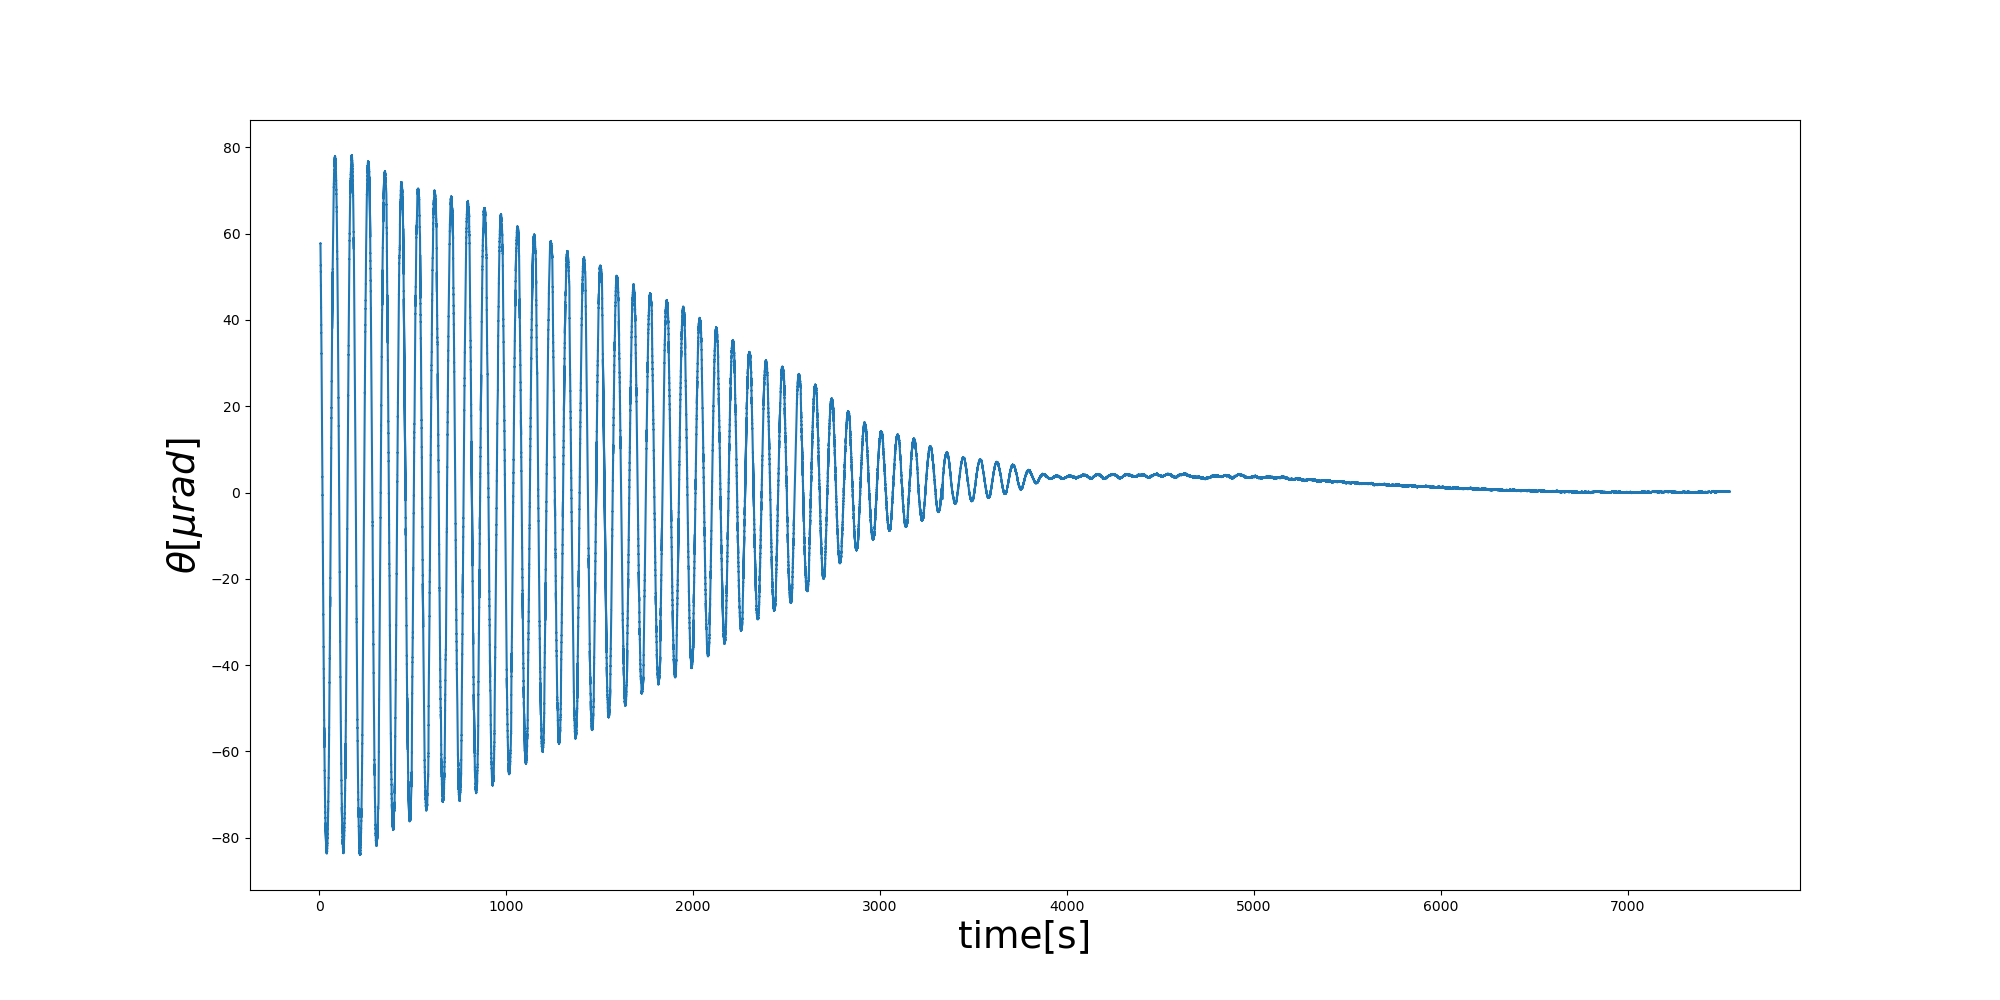
\includegraphics[width=0.7\textwidth,keepaspectratio]{measured oscillation angle.png}
	\end{center}
	\begin{itemize}	
		
		\item Damping accelerates as amplitude is getting smaller.
		\item Damping time of $3700[s]$ to damp  $ 60 [\mu rad] \rightarrow 10[\mu rad] $.
		\item Damping time of $250[s]$ to damp  $ 10 [\mu rad] \rightarrow 0.2[\mu rad] $.

						
	\end{itemize}
\end{frame}
\begin{frame}{Time integration}
	\begin{center}		
		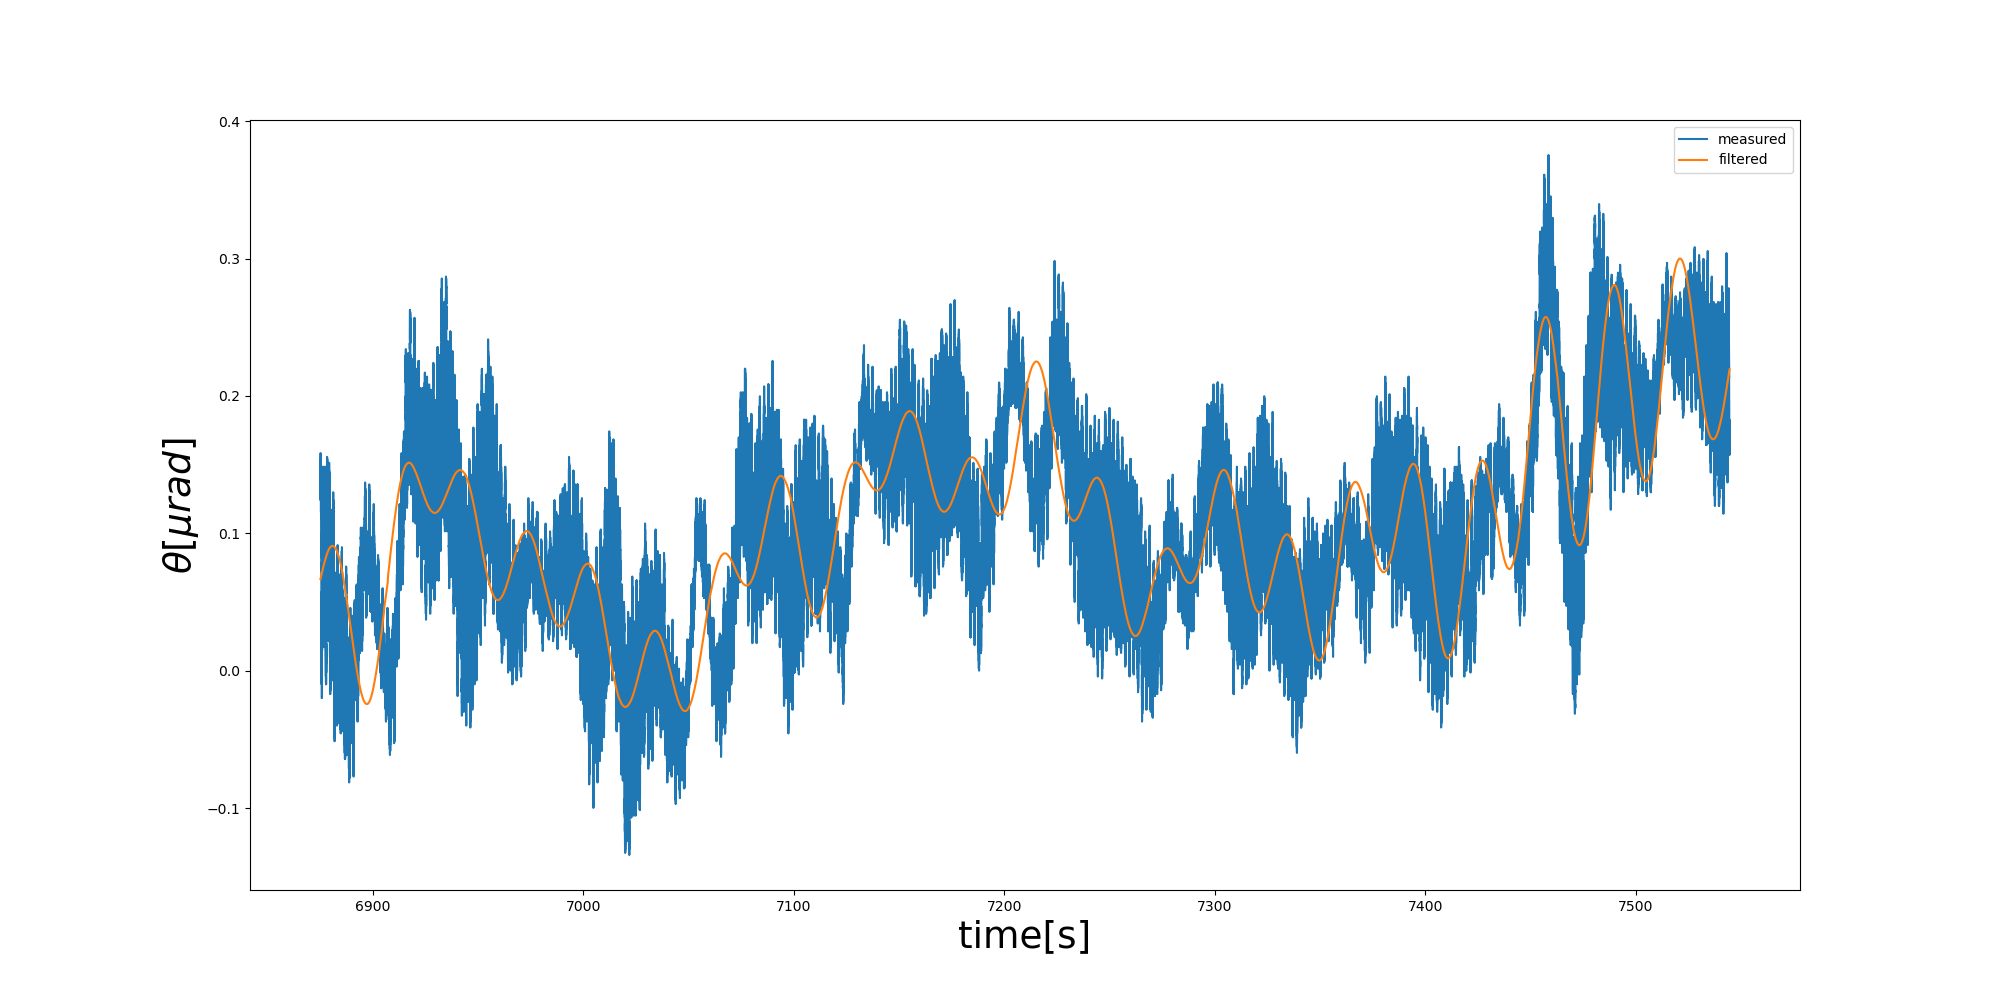
\includegraphics[width=0.7\textwidth,keepaspectratio]{measured oscillation angle1.png}
	\end{center}
	\begin{itemize}	
		\item Setup able to damp up to an amplitude of $0.05[\mu rad]$.
		\item RMS amplitude kept by the PID over time of $ 0.2 [\mu rad]$; which enables reducing uncertainty further more by time integration.	
		
						
	\end{itemize}
\end{frame}



\subsection{Noises}

\begin{frame}{\hypertarget{frame:Quality factor}{Quality factor}}
	\begin{center}		
		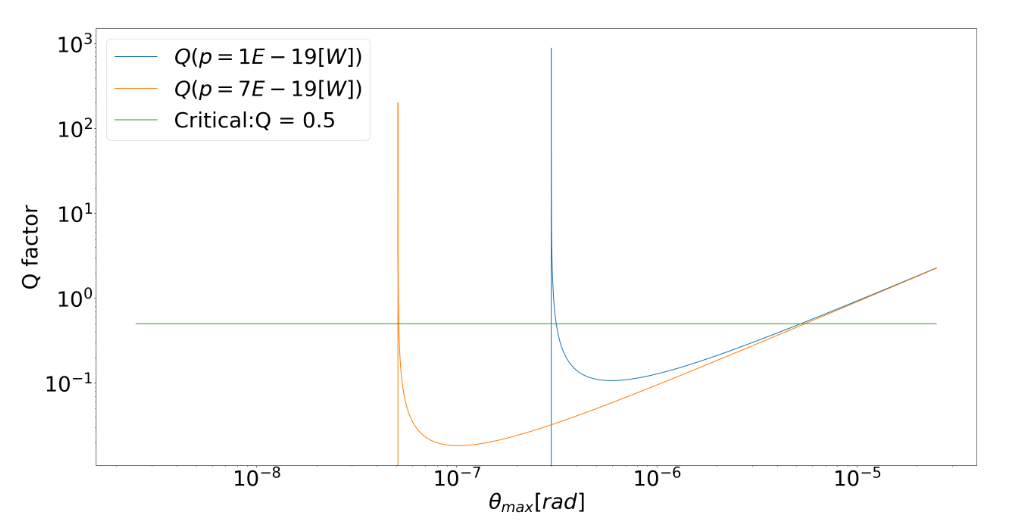
\includegraphics[width=0.5\textwidth,keepaspectratio]{Q factor.png}
	\end{center}
	\begin{itemize}	
		\item Quality factor describes how damped the oscillator.
		\item Noise and amplitude depended: $Q =  \frac{\pi\kappa\theta^2}{T(\frac{\theta\pi\tau}{T} -p)} $.
		\item $Q<0$; noise larger than damping - results with driving.
		\item Coupled noise estimation; from measured damped angle. 
		\item Noise estimation: $p \rightarrow \frac{ \theta\pi\tau}{T}$. 
	\end{itemize}
	\hyperlink{frame:Quality factor 1}{>>} 
\end{frame}

% frame 1
\begin{frame}{\hypertarget{frame:Environmental noises}{Environmental noises}}
	\begin{center}		
		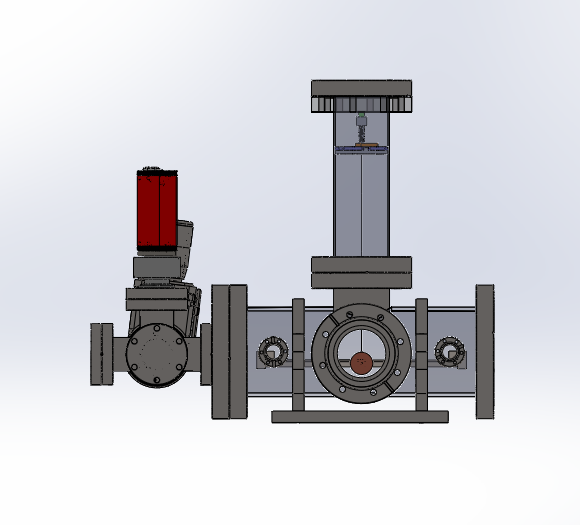
\includegraphics[width=0.4\textwidth,keepaspectratio]{total_chamber.png}
    \end{center}
	\begin{itemize}
		
		\item Environment gas cause pressure-dependent friction and noises (Brownian motion, acoustic waves, thermal flow).  
		\item Environmental black body radiation energy.
		\item Unknown Magnetic noise from the setup electronics.
		\item Estimated noise much smaller than calculated noise.				

			
	\end{itemize}
	\hyperlink{frame:Environmental noises 1}{>>} 
\end{frame}




\begin{frame}{\hypertarget{frame:Effective noise}{Effective noise}}
	\begin{center}		
		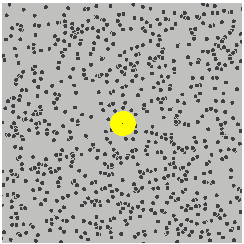
\includegraphics[width=0.3\textwidth,keepaspectratio]{random_motion1.jpg}
	\end{center}


	\begin{itemize}	
		
		\item Brownian motion and black body radiation are both treated as random particle collision processes ($\sqrt{N}$).
		\item Only net collision power affects the motion uncertainty.
		\item Coupled noise power composed only of net Brownian motion, net black body radiation and acoustic waves.  	 
					
	\end{itemize}
	\hyperlink{frame:Effective noise 1}{>>} 

\end{frame}


\begin{frame}{Resolution limit}
	
	\begin{itemize}
		\item Amplitude limited by Brownian uncertainty of $p=6.2\mu W$.
		\item Might allow to damp down to $\theta\approx 2\cdot 10^{-14}$ (from Q factor).
		\item Resolution limit proportional to damped amplitude $\theta$. 	
		\item Achieved if damping lowers temperature; $\theta = \sqrt{\frac{k_B T}{\kappa}}$.
				
	\end{itemize}
\end{frame}


\section{Summary and conclusion}


\begin{frame}{Study contribution}
	\begin{itemize}
		\item Improving sensitivity and integration time using active motion damping.
		\item With the right conditions, damping allows cooling up to the Brownian limit. 
		\item Possibility of achieving higher gravimetric measurement sensitivity than current state of the art.
		
	\end{itemize}
\end{frame}



Competitive method

\begin{frame}{Competitive method}
\begin{center}		
		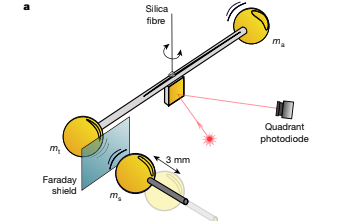
\includegraphics[width=0.3\textwidth,keepaspectratio]{nature.PNG}
	\end{center}

	\begin{itemize}
		\item Results were published in Nature at march 2021.

		\item Torsional pendulum placed inside vacuum and a faraday shield, with optical measurement of angular deflection.
		\item Measured down to $90 [mg]$ around spectral band of $12.7 [mHz]$, preventing high frequency nonlinear coupling.
		
	\end{itemize}
\end{frame}

\begin{frame}{Future study}
	\begin{itemize}
		
		\item PID not the best control algorithm; linear approximation. 
		\item Next stage would have non linear motion approximation.
		\item Goal of damping beyond room temperature uncertainty. 
	\end{itemize}
\end{frame}

\begin{frame}{Closing}
	\centering
	Thank you for your time. \\[12pt]
	
\end{frame}

\iffalse

\subsection[Basic Problem]{The basic problem that we have studed}

\begin{frame}{Slide Title \#1}
	\framesubtitle{Slide subtitle \#1}
	\begin{itemize}
		\item Use the \texttt{itemize} environment frequently.
		\pause
		\item Use short sentences and phrases.
		\pause
		\item In this presentation we use the \textbackslash{}\texttt{pause} macro.
	\end{itemize}
\end{frame}

\begin{frame}{Slide Title \#2}
	\begin{itemize}
		\item <1->You can define the order of appearance.
		\item <3->Like here.
		\item <2->This is the second item to appear.
	\end{itemize}
\end{frame}

\begin{frame}{Slide Title \#3}
	\begin{block}
		<1->{}
		\begin{itemize}
			\item Group without title.
			\item Appears for all slides.
		\end{itemize}
	\end{block}
	\begin{exampleblock}
		<2->{Group title}
		\begin{itemize}
			\item $e^{i\pi}=-1$.
			\item $e^{i\pi/2}=i$.
		\end{itemize}
	\end{exampleblock}
\end{frame}

%%
\subsection{Previous work}

\begin{frame}{Slide Title \#4}
	\begin{example}
		<1->First example. 
	\end{example}
	\begin{example}
		<2->Second example.
	\end{example}
\end{frame}

\begin{frame}{Slide Title \#5}
	\begin{center}
		Table example \\[12pt]
		\begin{tabular}{c||c|c|c|}
			& \textbf{col 1} & \textbf{col  2} & \textbf{col 3} \\
			\hline
			\hline
			\textbf{row 1} & 11 & 12 & 13 \\
			\hline
			\textbf{row 2} & 21 & 22 & 23 \\
		\end{tabular}
    \end{center}
\end{frame}

\begin{frame}{Slide Title \#6}
	\begin{center}
		Figure example \\[12pt]
		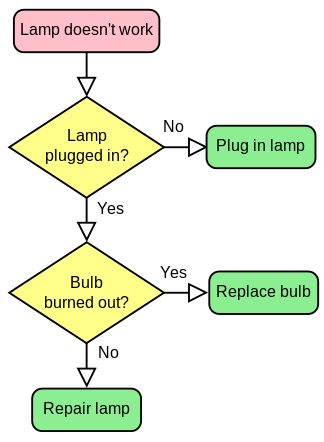
\includegraphics[width=0.35\textwidth,keepaspectratio]{LampFlowchart.png}
		\\
		\footnotesize(source: \textlatin{Wikipedia})
    \end{center}
\end{frame}

\begin{frame}{Slide Title \#7}
	\centering
	Math examples \\[12pt]
	\begin{equation}
        	B'=-\nabla \times E
	\end{equation}
	\begin{equation*}
        	E'=\nabla \times B - 4\pi j
	\end{equation*}
\end{frame}

%%%%
\section{Results / contribution}

%%
\subsection{Main results}

\begin{frame}{Summary}
   	\begin{alertblock}{Attention}
   		\textlatin{This is an important alert}
   	\end{alertblock}
\end{frame}

%
\subsection{Subsection title}

\begin{frame}{Summary}
	\begin{itemize}
		\item The \textcolor{red}{first main message} of our talk.
		\item The \textcolor{red}{second main message} of our talk.
		\item Maybe a \textcolor{red}{third message}, but ... no more.
	\end{itemize}
	\vskip0pt plus.5fill
	\begin{itemize}
		\item Conclusion.
	\end{itemize}
	\begin{itemize}
		\item Future work.
		\item Discussion.
	\end{itemize}
\end{frame}

\begin{frame}{References}
	\begin{thebibliography}{2}
		\beamertemplatebookbibitems
		\bibitem{Author1990}A.\ Author. \newblock\emph{Handbook of Everything}.\newblock
\textlatin{Some Press, \oldstylenums{1990}}.

		\beamertemplatearticlebibitems
		\bibitem{Someone2002}B.\ Author.\newblock On this and that\emph{.}
\newblock\emph{Journal on This and That}. 
\oldstylenums{2}(\oldstylenums{1}):\oldstylenums{50}--\oldstylenums{100}, 
\oldstylenums{2000}.
	\end{thebibliography}
\end{frame}
\fi





\section{Appendix}

% frame 2
\begin{frame}{\hypertarget{frame:Damped oscillator}{Damped oscillator}}

	\begin{center}		
		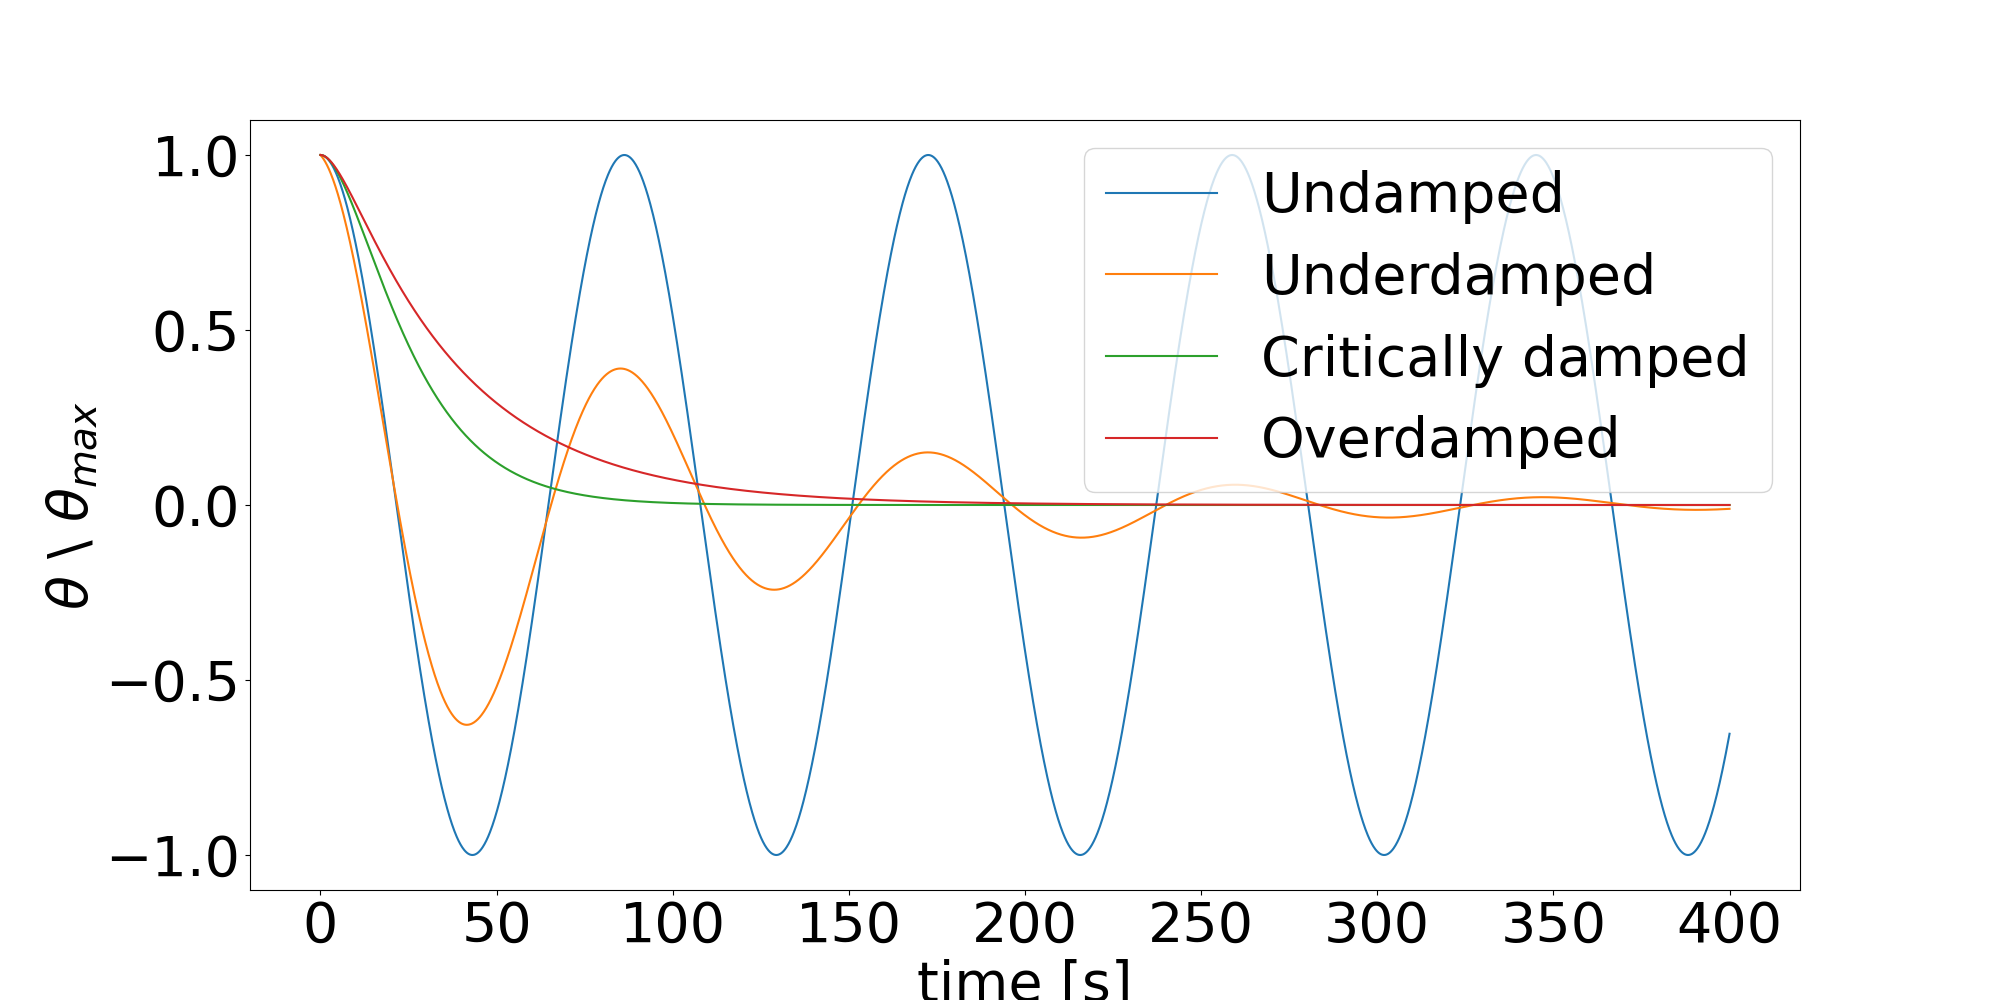
\includegraphics[width=0.55\textwidth,keepaspectratio]{damp.png}
    \end{center}
	\begin{itemize}	
		\item The damping ratio, $\xi$, determines the oscillator's motion: underdamped, critically damped or overdamped.
		\item Underdamped; oscillations amplitude decreases in time.
		\item Critically damped; exponential decay to equilibrium.
		\item Overdamped; exponential decay with longer damping time. 		
	\end{itemize}
	\hyperlink{frame:Harmonic oscillator}{<<} 
\end{frame}


% frame 3 - skip
\begin{frame}{\hypertarget{frame:Cavendish apparatus 1}{Cavendish apparatus}}
	\framesubtitle{Net torque}
	\begin{center}		
		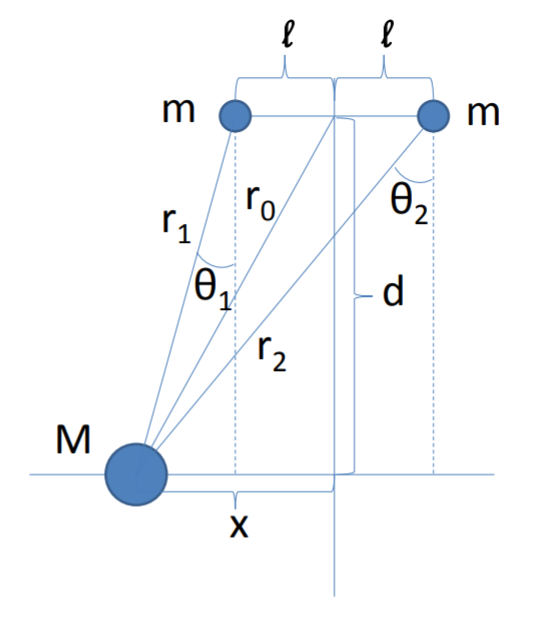
\includegraphics[width=0.25\textwidth,keepaspectratio]{Cavendish apparatus.PNG}
    \end{center}
	\begin{itemize}
		\item The net gravitational torque is the sum inverse torques, one from each mass: $\tau_g = l \cdot F(r_1) \cdot cos\theta_1 - l \cdot F(r_2) \cdot cos\theta_2$
		\item If $l<<d,x,r_0$ the net torque can be approximated to: $\tau_g =  \frac{6l^2GmMxd} {r_0^5} = \frac{6l^2GmM sin\theta cos\theta}{r_0^3}$
		\item Where the tilt angle is $\theta_1 \approx \theta_2 \approx \theta$.
	\end{itemize}
	\hyperlink{frame:Cavendish apparatus}{<<} 
\end{frame}
% frame 4 - skip
\begin{frame}{Cavendish apparatus}
	\framesubtitle{Approximation}
	\begin{center}		
		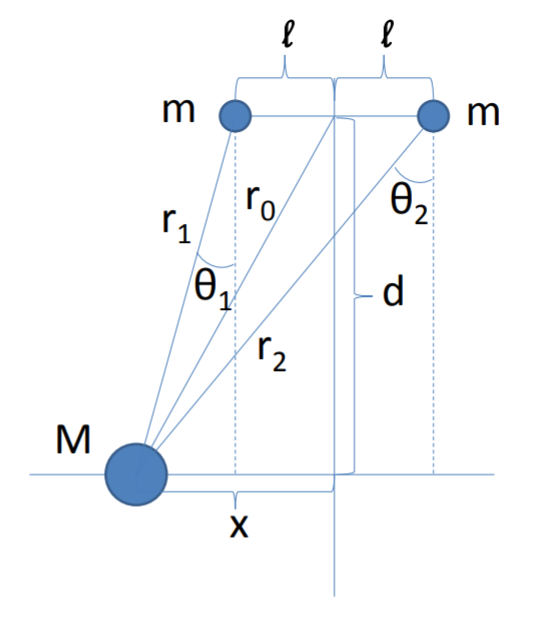
\includegraphics[width=0.2\textwidth,keepaspectratio]{Cavendish apparatus.PNG}
    \end{center}
	\begin{itemize}
		\item The net gravitational torque: $\tau_g =  l d GmM(\frac{1}{r_1^3} - \frac{1}{r_2^3})$.
		\item Defining the function: $h(l) = \frac{1}{(d^2 +(x-l)^2)^{3/2}}$.
		\item If $l<<d,x,r_0$ approximation: $h(l)-h(-l)\approx h'(0)\cdot 2l = \frac{6lx}{r_0^5}$.
		\item the net torque is proportional to the difference: $\tau_g = l d GmM[h(l)-h(-l)]\approx \frac{6l^2GmMxd} {r_0^5}$.
	\end{itemize}
	\hyperlink{frame:Cavendish apparatus}{<<} 
\end{frame}
% frame 5 - skip
\begin{frame}{Cavendish apparatus}
	\framesubtitle{Simple harmonic oscillator}
	\begin{center}		
		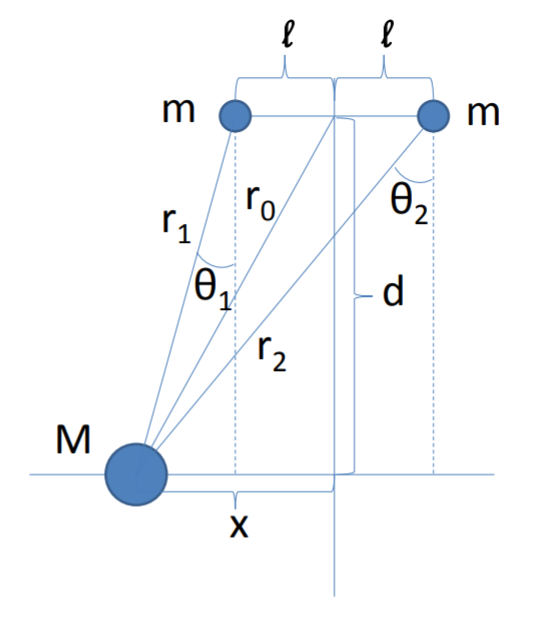
\includegraphics[width=0.25\textwidth,keepaspectratio]{Cavendish apparatus.PNG}
    \end{center}
	\begin{itemize}
		\item Assuming no damping force (simple harmonic motion).
		\item At equilibrium, the torques cancel each other out $\tau_g =  \kappa\theta$.
		\item The average equilibrium angle: $\overline{\theta} = \frac{\tau_g}{\kappa} \approx \frac{3GT^2cos\theta sin\theta}{4\pi^2 } \cdot \frac{M}{r_0^3}$.
		
	\end{itemize}
	\hyperlink{frame:Cavendish apparatus}{<<} 

\end{frame}

% frame 2 - skip
\begin{frame}{\hypertarget{frame:Environmental noises 1}{Environmental noises}}
	\framesubtitle{Pressure and temperature dependent noises}
	\begin{itemize}
		\item An ideal gas has negligible inter-particle interactions.
		\item Brownian motion cause random collisions. 
		\item The kinetic energy of the gas particles: $ N<E_k> = \frac{3}{2} PV$.
		\item Acoustic waves are propagating with power of $10^{-22}AP^2$.
		\item Heat flow is the exchange of thermal energy between physical systems. The net power is: $p= A P c_v \Delta T \sqrt{\frac{M}{RT}} $.
		\item Net power from black body radiation is $p= A \sigma\epsilon[ T^4- T_0^4]$.
		
	\end{itemize}
	\hyperlink{frame:Environmental noises}{<<} 
\end{frame}


% frame 2 - skip
\begin{frame}{\hypertarget{frame:Environmental noises 2}{Environmental noises}}
	\framesubtitle{Friction}
	\begin{itemize}
		\item Friction, caused by drag force, decreases with pressure.		
		\item At higher pressures (turbulent flow); $F = -b(P)\cdot v^2 $.
		\item At lower pressures (gas with laminar flow), the drag force is given by Stokes' law: $F_{drag} =  -b(P)\cdot v$.	
		
	\end{itemize}
	\hyperlink{frame:Environmental noises}{<<} 
\end{frame}

% frame 5
\begin{frame}{\hypertarget{frame:Proportional–integral–derivative (PID) controller 1}{Proportional–integral–derivative (PID) controller}}
	\framesubtitle{PID response}
	\begin{center}		
		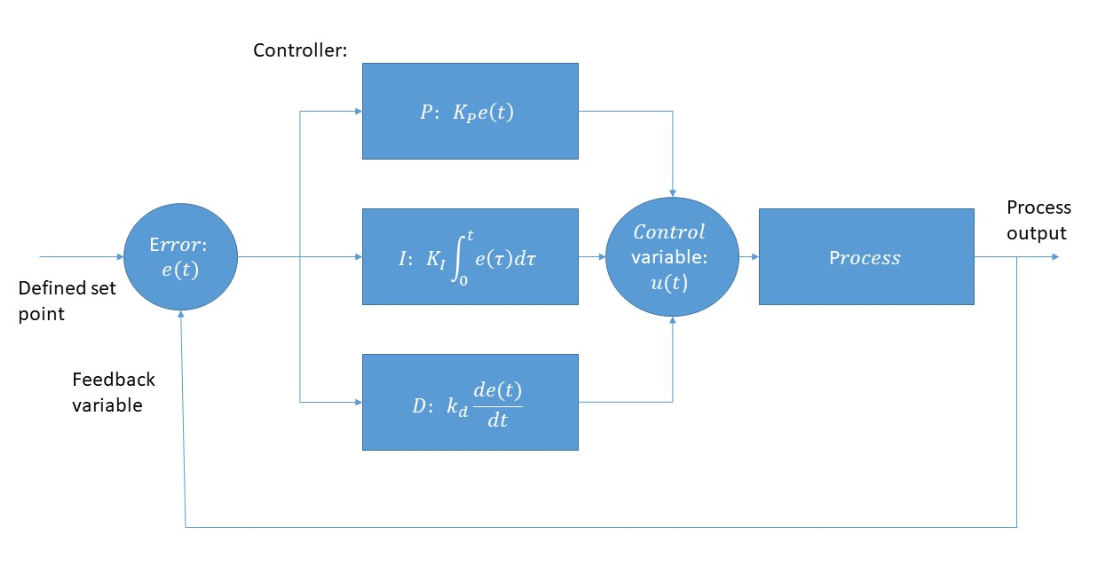
\includegraphics[width=0.6\textwidth,keepaspectratio]{pid_diagram_powerpoint.jpg}
    \end{center}
	\begin{itemize}
		\item The controller continuously calculates error from set point. 
		\item Each response is modulated by a tunable gain. 
		\item Output: $u(t) = K_P e(t)+K_I\int_{0}^{t}e(\tau)d\tau+K_D\frac{de(t)}{dt}$		
	\end{itemize}
	\hyperlink{frame:Proportional–integral–derivative (PID) controller}{<<} 
\end{frame}


\begin{frame}{\hypertarget{frame:Radiation tourqe 1}{Radiation tourqe}}
\framesubtitle{Radiation pressure}
	\begin{center}		
		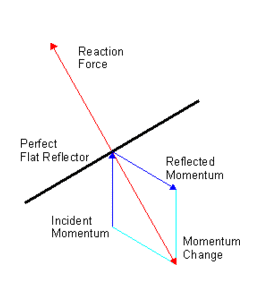
\includegraphics[width=0.2\textwidth,keepaspectratio]{radiation.PNG}
    \end{center}

	
	\begin{itemize}		
		\item Surface pressure of a light beam causes force.
		\item The force depend on the relative angle, surface reflectance and absorbance and the incident light power.
		\item With light perpendicular to a reflective surface $F  \approx\frac{2\eta\Theta}{{c}} $.
		
	\end{itemize}
	\hyperlink{frame:Radiation tourqe}{<<} 
\end{frame}

% frame 2 - skip
\begin{frame}{\hypertarget{frame:Measurement uncertainty 1}{Measurement uncertainty}}
	\begin{itemize}
		\framesubtitle{Fundamental limits}
		\item Basic energy level quantum uncertainty: $\delta\theta= \sqrt{\frac{\hslash\omega}{2\kappa}} \approx 10^{-16} [rad]$
		\item Quantum uncertainty due to thermal energy: $\delta\theta = \sqrt{\frac{k_B T}{\kappa}} \approx 4\cdot 10^{-8} [rad]$.
		\item Shot noise limit: $\delta\theta = \frac{1}{4\sqrt{2}\pi}\frac{\lambda}{L\sqrt{N}} \approx 10^{-14} [\frac{rad}{Hz}]$.
		
	\end{itemize}
	\hyperlink{frame:Measurement uncertainty}{<<}
\end{frame}


\begin{frame}{\hypertarget{frame:LED PWM setup 1}{LED PWM setup}}
	\framesubtitle{Arduino microcontroller}
	\begin{center}		
		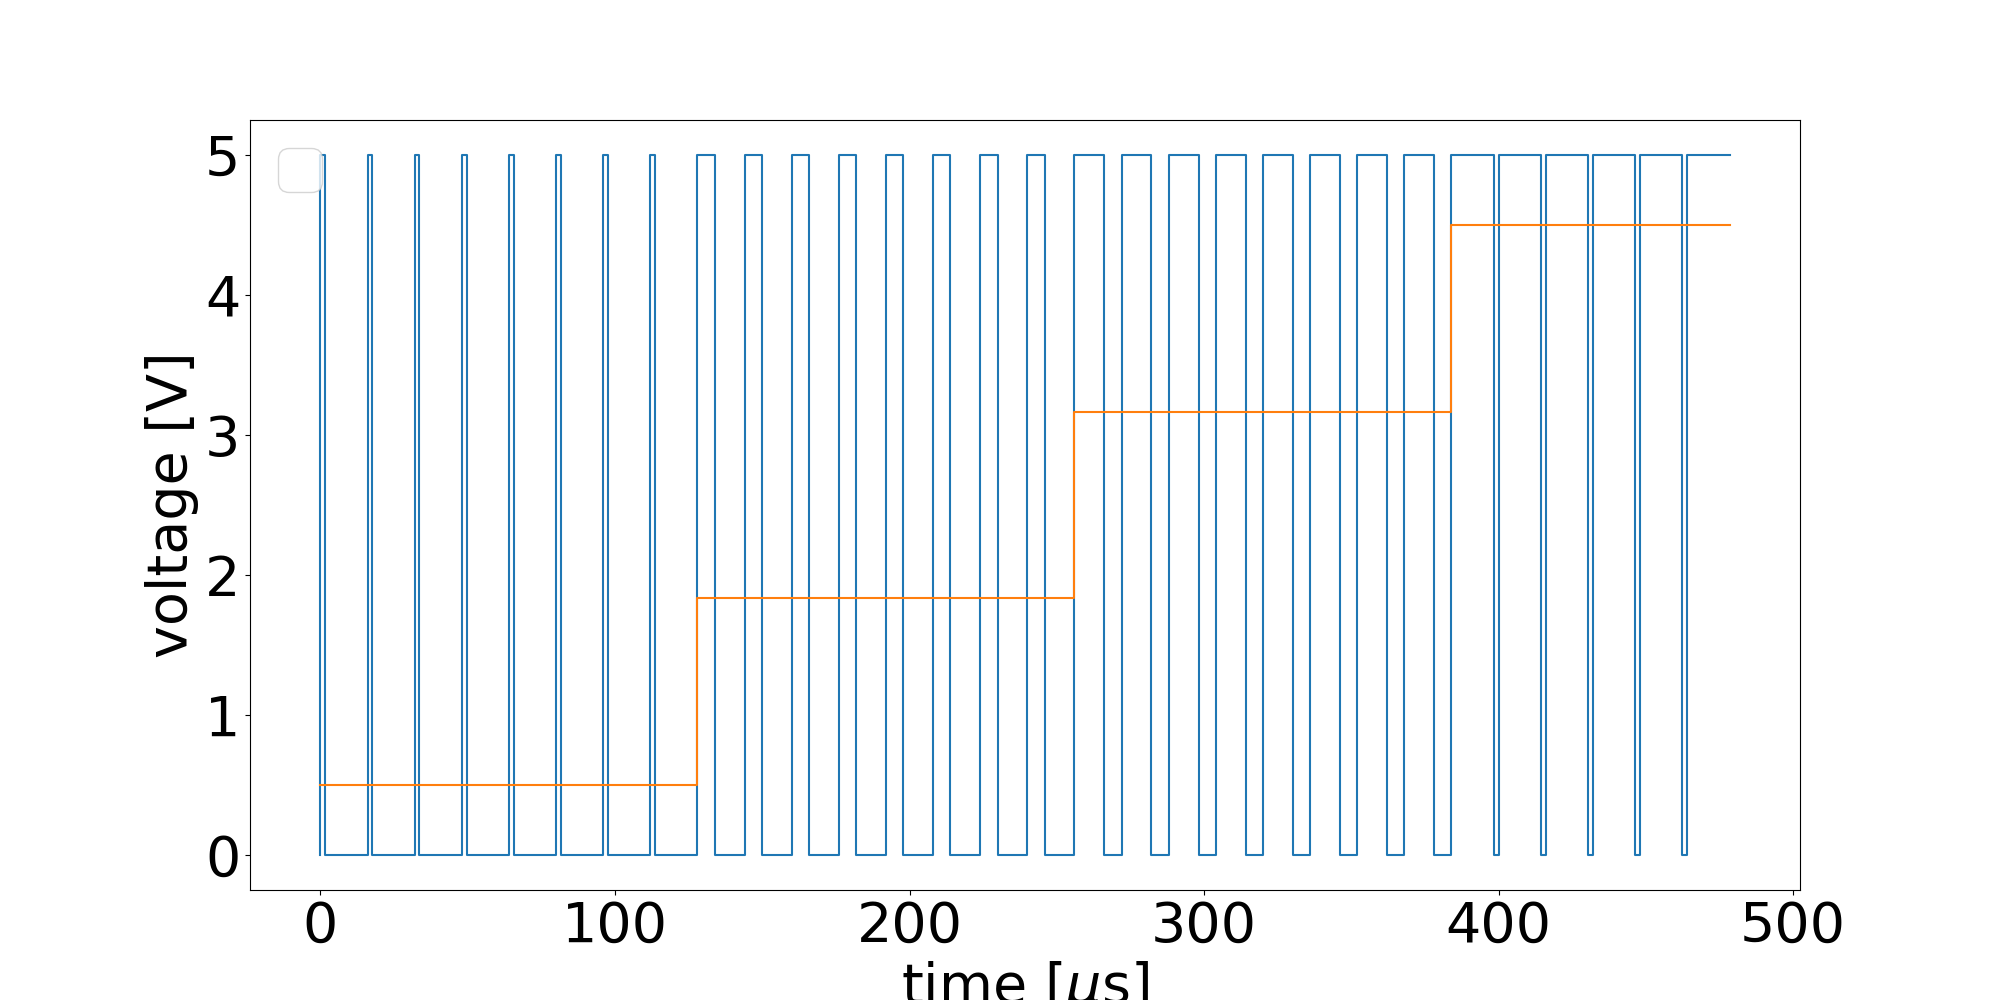
\includegraphics[width=0.55\textwidth,keepaspectratio]{duty_cycle.png}
	\end{center}
	\begin{itemize}		
		\item Inexpensive 8-bit microcontroller with Pulse Width Modulation (PWM) analog outputs.
		\item Fast switching of digital signal results with analog signal.
		\item Analog signal depended on duty-cycle: $V(t) =  \frac{V_d}{100}\cdot D(t)$.
		\item Modulation limited by clock frequency: $f_{PWM} \approx 500[Hz]$.
	\end{itemize}
	\hyperlink{frame:LED PWM setup}{<<} 
\end{frame}

\begin{frame}{\hypertarget{frame:Quality factor 1}{Quality factor}}
	\framesubtitle{Calculation}
	\begin{center}		
		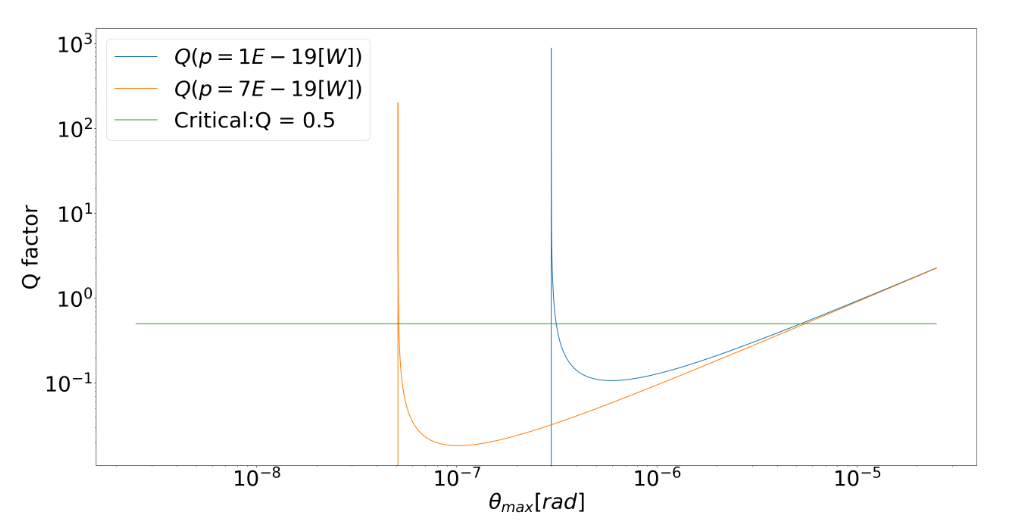
\includegraphics[width=0.5\textwidth,keepaspectratio]{Q factor.png}
	\end{center}
	\begin{itemize}			
		\item Ratio of the energy stored to dissipated per cycle.
		\item The difference of PID work and coupled noise power. 
		\item Noise and amplitude depended: $Q =  \frac{2\pi\cdot(\frac{\kappa\cdot\theta_{max}^2}{2})}{\int_0^T[\tau(t)\cdot\dot{\theta}(t) - p]dt} $
					
	\end{itemize}
	\hyperlink{frame:Quality factor}{<<} 

\end{frame}


\begin{frame}{\hypertarget{frame:Effective noise 1}{Effective noise}}
	\framesubtitle{Calculated noises}
	\begin{itemize}	
		\item Thermal flow: $p=0.083[W]$.
		\item Black body radiation: $p=0.121[W]$.
		\item Brownian motion: $p=6.2\cdot 10^{-6}[W]$.
		\item Acoustic waves: $p=1.1\cdot 10^{-28}[W]$.
		\item New estimated noise: $p=1\cdot 10^{-19} - 7\cdot 10^{-19}[W]$.
					
	\end{itemize}
	\hyperlink{frame:Effective noise}{<<} 
\end{frame}
\end{document}